\documentclass[a4paper]{article}

%% Language and font encodings
\usepackage[english]{babel}
\usepackage[utf8x]{inputenc}
\usepackage[T1]{fontenc}

%% Sets page size and margins
\usepackage[a4paper,top=3cm,bottom=2cm,left=3cm,right=3cm,marginparwidth=1.75cm]{geometry}

%% Useful packages
\usepackage{amsmath}
\usepackage{graphicx}
\usepackage{titling}
\usepackage[colorinlistoftodos]{todonotes}
\usepackage[colorlinks=true, allcolors=blue]{hyperref}
\usepackage{listings}
\newcommand{\CenterCell}[1]{\multicolumn{1}{|c|}{#1}}
\usepackage{fullpage}
\usepackage{times}
\usepackage{url}
\usepackage{cite}
%\usepackage{boxit}
\usepackage{alltt}
\usepackage{booktabs}
\usepackage{xspace}
%%%
%%%% From projects/papers/splash13-red/{main,macros}.tex
%\usepackage{sbfig}
\newcounter{sbfgcnt}

\renewcommand{\thesbfgcnt}{(\alph{sbfgcnt})}

\def\sbfg#1{%
\refstepcounter{sbfgcnt}
\begin{flushleft}
  \footnotesize
  \hrule
  \vskip2pt
  \hspace{2pt}\thesbfgcnt\xspace #1
  \vskip2pt
  \hrule\hrule
\end{flushleft}
% \vskip-10pt
}

\def\sbtbl#1{%
\refstepcounter{sbfgcnt}
\thesbfgcnt\xspace #1

}
\newcommand{\CodeIn}[1]{\begin{footnotesize}\texttt{#1}\end{footnotesize}}
\newcommand{\figref}[1]{Figure~\ref{#1}}     % for use in text
\newcommand{\subfigref}[2]{Figure~\ref{#1}\ref{#2}}
\newcommand{\Figref}[1]{Figure~\ref{#1}}   % for start of sentence

%\definecolor{RedCommentColor}{rgb}{0.247, 0.498, 0.273}
\definecolor{RedCommentColor}{HTML}{669966}
\definecolor{RedStringColor}{rgb}{1, 0, 0}
%\definecolor{RedKeywordColor}{rgb}{0, 0, 0.6}
\definecolor{RedKeywordColor}{HTML}{990033}
%\definecolor{RedBkgColor}{rgb}{0.98, 0.98, 0.98}
\definecolor{RedBkgColor}{HTML}{FFFF00}
\definecolor{RedTypeColor}{HTML}{336699}
%\def\myemphstyle{\color{blue!40!black}\bfseries}
\def\myemphstyle{\color[HTML]{336699}\bfseries}

% \definecolor{RedCommentColor}{rgb}{0, 0, 0}
% \definecolor{RedStringColor}{rgb}{0, 0, 0}
% \definecolor{RedKeywordColor}{rgb}{0, 0, 0}
% \definecolor{RedBkgColor}{rgb}{1, 1, 1}
% \def\myemphstyle{}
	
%\definecolor{RedCommentColor}{rgb}{0.247, 0.498, 0.273}
\definecolor{RedCommentColor}{HTML}{669966}
\definecolor{RedStringColor}{rgb}{1, 0, 0}
%\definecolor{RedKeywordColor}{rgb}{0, 0, 0.6}
\definecolor{RedKeywordColor}{HTML}{990033}
%\definecolor{RedBkgColor}{rgb}{0.98, 0.98, 0.98}
\definecolor{RedBkgColor}{HTML}{FFFF00}
\definecolor{RedTypeColor}{HTML}{336699}
%\def\myemphstyle{\color{blue!40!black}\bfseries}
\def\myemphstyle{\color[HTML]{336699}\bfseries}

% \definecolor{RedCommentColor}{rgb}{0, 0, 0}
% \definecolor{RedStringColor}{rgb}{0, 0, 0}
% \definecolor{RedKeywordColor}{rgb}{0, 0, 0}
% \definecolor{RedBkgColor}{rgb}{1, 1, 1}
% \def\myemphstyle{}

% \newcommand{\Hilight}{\makebox[0pt][l]{\color{gray}\rule[-3pt]{0.80\linewidth}{9pt}}}
% \lstdefinelanguage{pseudo}{
%   morekeywords={if,else,return,true,false,public,static,void},
%   keywordstyle=\bfseries,
%   lineskip=-0.1em,
%   numbers=none,
%   numberstyle=\jnumberstyle,
%   numbersep=4pt,
%   basicstyle=\scriptsize,
%   basicstyle=\jbasicstyle,
%   breaklines=true,
%   breakautoindent=true,
%   tabsize=2,
%   columns=fullflexible,
%   morecomment=*[l][\textsl]{//},
%   mathescape=true,
% }
% \newcommand{\code}[1]{{\ifmmode{\mathtt{#1}}\else$\mathtt{#1}$\fi}}


\lstdefinelanguage{redlisting}{
  keywords={%
     abstract_record, abstract_machine, record, machine, do, end, event, data, set, seq, let, entity, message, some, all, one, lone, no, requires, ensures, new, class, in, from, to, case, response, params, send, receive, if, then, else, when, unless, fail, def, policy, principal, restrict, reject, refs, owns, fields, super},
  sensitive=true,  % case sensitive
  emph={Client,User,Server,AuthUser,AuthServer,AuthClient,Msg,ChatRoom,String,CreateRoom,JoinRoom,SendMsg,HideUserPrivateData,FilterChatRoomMembers,SignIn,SignOut,Register,Unregister,WebClient,WebServer,Text,UpdateTables,ActiveRecord,Base,Red,Model,Record,Migration},
  emphstyle={\myemphstyle},
  morecomment=[l]{\#},
  morecomment=[s]{/*}{*/},
  morestring=[b]",
  showstringspaces=false, 
  numbers=none,
  firstnumber=0,
  numberstyle=\tiny,
  % backgroundcolor=\color[HTML]{FFFF00},
  stepnumber=5,
  basicstyle=\tiny\ttfamily,
  commentstyle=\itshape\color{RedCommentColor},
  keywordstyle=\bfseries\color{RedKeywordColor},
  stringstyle=\itshape\color{RedStringColor},
  ndkeywordstyle=\bfseries,
  frame=single,
}

\lstnewenvironment{redLines}[1][]{%
  \lstset{language=redlisting,
    floatplacement={tbp},captionpos=b,
    frame=lines,xleftmargin=2pt,xrightmargin=2pt,#1}}{}
\lstnewenvironment{redlisting}[1][]{%
  \lstset{language=redlisting,
    floatplacement={tbp},captionpos=b,
    xleftmargin=2pt,xrightmargin=2pt,#1}}{}


% \pretitle{\begin{center}\fontsize{18bp}{18bp}\selectfont}
%     \posttitle{\par\end{center}}
% \preauthor{\begin{center}\fontsize{14bp}{14bp}\selectfont}
%     \postauthor{\par\end{center}\vspace{24bp}}
\begin{document}
\title{Scalable programming for interactive mobile applications}
% \author{Atul Sandur}
\predate{}
\date{}
\postdate{}

\maketitle

\begin{abstract}
Mobile devices are becoming increasingly pervasive with smartphones making up a significant portion of those devices. Applications running on these devices are complex and becoming highly distributed in nature~\cite{7879258}. Advancements in mobile development frameworks have made it easier to program standalone applications, but developing an entire system with applications running on mobile devices backed by cloud servers and storage still remains a challenge. Work such as Meteor~\cite{Meteor} and Sunny~\cite{Milicevic} makes writing such applications easier. But it falls short of providing scalability and fault tolerance guarantees across a broad range of applications. So we leverage Sunny infrastructure to provide a distributed runtime that spans mobile and cloud services, and is also much more fluid in nature. It can provide consistency/latency guarantees, mobility of components across different physical resources, fault tolerance characteristics and performance/energy SLAs for broad range of mobile applications. We propose a translation mechanism from model-based program specifications to a friendly user interface on the one hand, and a scalable actor based system which relieves the mobile application developer from dealing with concurrency and scalability issues in a distributed setting. We demonstrate the capabilities of our proposed framework by developing a real world chat application. 
\end{abstract}

\section{Introduction}

Over a third of the world's population owns a smartphone \cite{smartphonestat} and that number is only expected to grow over the next decade. The era of social networking, online banking/retail and distributed computing have led to increasing complexity in the programming of applications running on smartphones. Interactiveness and multi-user experience are essential features in these applications and they result in complexity in programming due to the following reasons \cite{Milicevic}:
\begin{itemize}
\item \emph{distributed} architecture of multiple servers on the cloud, interacting with millions of clients on different smartphone platforms
\item \emph{abstraction gap} between the problem-domain level (high-level, event-driven) and implementation-level (low-level messaging, queues, schedulers and asynchronous callbacks)
\item \emph{mobility of clients} causing intermittent network connectivity issues and hence non-deterministic latencies in interaction with server 
\item \emph{failures} which may cause applications to lose state or suffer from performance degradations
\item shared \emph{data consistency}
\item \emph{concurrency} issues such as data races, atomic violations and deadlocks
\end{itemize}

Abstraction mismatches not only distract the programmer from focusing on the essential task at hand, but also prevents reasoning about a correct and robust system that addresses the issues enumerated above. We leverage an existing model-based programming paradigm~\cite{Milicevic} for developing interactive, event-driven systems and develop a \emph{translation and runtime environment} for scalably executing these programs using the actor model~\cite{actors}. This reduces the maintenance and debugging costs for distributed mobile applications, relative to the development efforts required today for building web applications. \\

Mobile application development involves two separate concerns- interaction designer on the one hand, wants to easily and rapidly develop user-level behaviors that can be expressed directly and succinctly. On the other hand, there is the system architect who wants to achieve scalable performance and reliability, by directly controlling how user-level tasks are mapped to computational resources. In order for both parties to be able to focus on their own concerns and ignore those of others, a precise but straightforward semantic mapping is required between languages for expressing user level and architecture level behaviors. \\

At the user level, the language can support declaration of typed relational data and atomic events that read and write the data (such as the one described in~\cite{Milicevic}). The data store is abstractly regarded as if it were global and centralized. In the implementation, it may be distributed and mapped to different representations (relational databases, key-value stores, etc.). At the architecture level, the application is defined using the actor model, a distributed computational model in which all communication is mediated by messages between actors. This hides from the programmer, complexities such as network communication between clients/servers, concurrency and races, persistent storage and coordination of events, and delegates it to the underlying runtime environment. \\

In order to provide the programmer with ability to easily write scalable mobile applications by leveraging the actor model~\cite{actors}, this work is intended to make the following contributions: 
\begin{itemize}
\item Designing the translation mechanism from high level language that uses relational/event model to user interface (GUI) on the one hand and corresponding actors on the other, for backend processing and data consistency management.  
\item Design a generic interface between events generated from user interactions with application GUI to messages triggering actor behaviors for performing the necessary computations.
\item Provide the runtime on smartphones, for executing SALSA~\cite{Varela:2001:PDR:583960.583964} based actor applications
\item Demonstrate the capabilities of our system using a chat room application
\end{itemize}
% provides can leverage cloud resources in a scalable way, while simplifying abstractions for developers and consequently development effort.

Note that the translation to actors in the backend enables integration with frameworks such as geo-distributed Orleans~\cite{orleans} where parameters like consistency and latency become configurable. It also helps leverage all the benefits of Orleans such as the geo-distributed nature of services, fault tolerance and configurable consistency/latency parameters. 

\section{Motivating example- chat room application}
To illustrate our approach on a concrete example, we
consider a chat room application. This example provides a skeleton for a number of cloud based mobile applications that involve distributed communication, including social media sites and popular online games. \\

Let's say users in our chat room application can join chat rooms, read messages and write messages. As far as the user is concerned, the application can be understood as consisting of a large building containing many rooms. The user can enter a room, and on doing so, will find a large whiteboard onto which messages can be written. From this user’s perspective, the state of the application is just a set of rooms, a set of users, each of which can be inside one or more rooms, and for each room, a sequence of messages inscribed on the room’s whiteboard. The observed behavior is simply a sequence of events in which users enter and leave rooms, and write messages on boards. These events are instantaneous, so there are no questions about conflicts between users attempting to write to the same board, for example. Formally then, from the user’s perspective, there is a single global state (consisting of rooms, boards and users) and a collection of events that can be performed by users. There is potentially no parallelism nor distribution.\\ 

From a system implementor’s perspective, however, a very different picture is needed. The state must be geo-distributed across many client machines; the implementor’s challenge is to give the users the illusion
that there is a single global state, when in fact state updates will not be propagated to clients in perfect synchrony, so that were a user to be able to observe two clients, she might see slightly different views.
Moreover, messages written to a board from different clients may be subject to varying delays. But again, these issues are neither observable nor of interest to the end users (so long as the delays are sufficiently short, of course). Likewise, while the user may view the system as having a single sequential execution of a stream of events, for the system implementor it will be essential to parallelize the application in order to make it scale, mapping the tasks (reading incoming messages, updating the boards, sending outgoing messages, maintaining presence information, etc.) to threads in a design that reflects an understanding of what kind
of load will be presented, how computationally intensive each task is, how messages will be spread across boards, and so on. \\ 

Since the clients may be joining chat rooms from across the world, geo-distribued servers must be hosted to provide latency guarantees. Furthermore failures of one of the chat room server machines may require migration of the data and associated computation to a different location. Multimedia content embedded in chat window and streamed via the client interface may need to be processed before rendering the frames on smartphone display. Depending on the processing required and the power/computational resources available on the smartphone, one may choose to offload the processing to a remote server. \\

Today, an application developer will have to address all of the aspects of the application discussed above, at once. At the user level, she will need to design the interactions that users will experience in terms of the event model. But this alone will not suffice; she will have to back up this view with a low-level implementation that takes account of the
concurrency, distribution and fault tolerance aspects. Frameworks such as Sunny, Rails and Django combine many of these features but either at the expense of constraining the kinds of applications that can be easily built (for example, treating communications initiated by the server as a special category of “push” messages that require special features, and by limiting the use of concurrency in handling requests) or not fully enabling the scalability, consistency and fault tolerance guarantees that come with computational models such as actors in a geo-distributed environment.

\subsection{Sample user level code}
We now look at how a user can express the different functionalities of a chat room, using a simple high level language. We assume that anyone can create a chat room (provided that a room with the same name does not already exist) and that the existing rooms are public, so anyone can join and subsequently write messages to a room’s board. With most applications of this kind, the web GUI must be responsive and interactive, automatically refreshing parts of the screen whenever something important happens (e.g., a new message is received), without reloading the whole page. 

\begin{figure*}[t!]
\setcounter{sbfgcnt}{0}
\begin{minipage}[t]{.60\linewidth}
\vspace{-5pt}
\begin{minipage}[t]{.45\linewidth}
\vskip0pt

\begin{redlisting}
record User < AuthUser do
  # inherited fields
  #   name: String, 
  #   email: String, 
  #   pswd_hash: String,
  refs status: String
end
\end{redlisting}
\end{minipage}
\hfill
\begin{minipage}[t]{.50\linewidth}
\vskip0pt
\begin{redlisting}
record Msg do
  refs text: Text, 
       sender: User
end



\end{redlisting}
%\end{minipage}
%\hfill
%\begin{minipage}[t]{.36\linewidth}
\vskip0pt
\begin{redlisting}
record ChatRoom do
  refs name: String, 
       members: (set User)
  owns messages: (seq Msg)
end
 

\end{redlisting}
\end{minipage}
\end{minipage}
\hfill
\begin{minipage}[t]{.3\linewidth}
\sbfg{network model\label{sbfg:entities}}
\vspace{-5pt}
\begin{redlisting}
machine Client < AuthClient
  refs user: User
end

machine Server < AuthServer
  owns rooms: (set ChatRoom)
end
\end{redlisting}
\end{minipage}
\vspace{-5pt}
\vskip5pt
\sbfg{event model\label{sbfg:ircevents}}
\vspace{-5pt}
\begin{minipage}[t]{.34\linewidth}
\vskip0pt
\begin{redlisting}
event CreateRoom do
  from client: Client 
  to   serv: Server
  
  params roomName: String
  
  requires {
    client.user    && 
    roomName       && 
    roomName != "" &&
    !serv.rooms.
      find_by_name(roomName)
  }
  
  ensures {
    room = ChatRoom.create
    room.name = roomName
    room.members = [client.user]
    serv.rooms << room
  }
end
\end{redlisting}
\end{minipage}
\hfill
\begin{minipage}[t]{.34\linewidth}
\vskip0pt
\begin{redlisting}
event JoinRoom do
  from client: Client
  to   serv: Server
  
  params room: ChatRoom
  
  requires {
    u = client.user
    client.user &&
    !room.members.include?(u)
  }
  
  ensures {
    room.members << client.user
  }
end




\end{redlisting}
\end{minipage}
\hfill
\begin{minipage}[t]{.30\linewidth}
\vskip0pt
\begin{redlisting}
event SendMsg do
  from client: Client
  to   serv: Server
  
  params room: ChatRoom, 
         msgText: String
  
  requires {
    client.user &&
    room.members.include?
      (client.user)
  }
  
  ensures {
    msg = Msg.create
    msg.text = msgText
    msg.sender = client.user
    room.messages << msg
  }
end

\end{redlisting}
\end{minipage}
\vspace{-5pt}
\vskip5pt
\sbfg{security model\label{sbfg:ircpoly}}
\vspace{-5pt}
\begin{minipage}[t]{.45\linewidth}
\vskip0pt
\begin{redlisting}
policy HideUserPrivateData do
  principal client: Client
  
  # restrict access to passwords
  # except for owning user
  restrict User.pswd_hash.unless do |user|
    client.user == user
  end

  # restrict access to status messages to
  # users who share at least one chat room
  # with the owner of that status message
  restrict User.status.when do |user| 
    client.user != user &&
    ChatRoom.none? { |room| 
      room.members.include?(client.user) &&
      room.members.include?(user)
    }
  end
end
\end{redlisting}
\end{minipage}
\hfill
\begin{minipage}[t]{.54\linewidth}
\vskip0pt
\begin{redlisting}
policy FilterChatRoomMembers do
  principal client: Client

  # filter out anonymous users (those who have not 
  # sent anything) from the 'members' field
  restrict ChatRoom.members.reject do |room, member|
    !room.messages.sender.include?(member) &&
    client.user != member
  end
end

\end{redlisting}
\end{minipage}
\caption{A model of a simple chat room application, written in 
our prototype modeling notation.}
\label{fig:spec}
\end{figure*}


\Figref{fig:spec} shows the application's user-level code. The code
consist of several different \emph{models} of the system, describing
different aspects.  The \emph{data model} consists of a \CodeIn{User}
record (which specializes a library \CodeIn{AuthUser} record and adds a
status field), a \CodeIn{Msg} record (where each message has a textual
body and a sender), and a \CodeIn{ChatRoom} record (each room has a name,
a set of participating users, and a sequence of messages that have
been sent).  These fields are defined using the \CodeIn{refs} and
\CodeIn{owns} keywords: the former denotes aggregation (simple
referencing, without any constraints), and the latter denotes
composition (implying that (1) when a record is deleted, all owned
records should be deleted, and (2) no two distinct records can point
to the same record via the same owned field).

The \emph{network model} in this example consists of two machines, namely \CodeIn{Server} and \CodeIn{Client}.  The \CodeIn{Client} machine has a corresponding \CodeIn{User}, whereas the \CodeIn{Server} machine maintains a set of active \CodeIn{ChatRoom}s.  They respectively inherit from the library \CodeIn{AuthClient} and \CodeIn{AuthServer} machines, to bring in some fairly standard (but library-defined, as opposed to built-in) user management behavior, such as new user registration, sign-in and sign-out events, etc.

To implement the basic functionality of the chat room, we define an \emph{event model} with three event types: \CodeIn{CreateRoom}, \CodeIn{JoinRoom}, and \CodeIn{SendMsg}, as shown in \figref{fig:spec}\ref{sbfg:ircevents}.

Each event has an appropriate precondition (given in the  \CodeIn{requires} clause) that checks that the requirements for the event are all satisfied before the event may be executed.  For instance,
events \CodeIn{CreateRoom}, \CodeIn{JoinRoom}, and \CodeIn{SendMsg} all require that the user has signed in (\CodeIn{client.user} is non-empty), \CodeIn{SendMsg} requires that the user has joined the room, etc.

A specification of the effects of an event (given in the \CodeIn{ensures} clause) is concerned only with updating relevant data records and machines to reflect the occurrence of that event. For example, the effects of the \CodeIn{JoinRoom} event amount to simply adding the user requesting to join the room to the set of room members; the runtime system will make sure that this update is automatically pushed to all clients currently viewing that room. Actions such as updating
the user interface are specified elsewhere, independently of the event model; this is a key to achieving separation of concerns.

By default, all fields in our models are public and visible to all machines in the system. To restrict access, we need to define a security policy as a collection of declarative rules such as the one shown in \Figref{fig:spec}. We will not however get into the details of these rules since the security aspect is out of scope for this report. 

\section{Architecture level language}
As mentioned earlier, we use the actor~\cite{actors} model of computation for processing at the architecture level. Actors provide a flexible model of concurrency for open distributed systems. Actors can be used to model traditional functional, procedural, or object oriented systems. Actors are independent, concurrent entities that communicate by exchanging messages asynchronously. Each actor encapsulates a state and a thread
of control that manipulates this state. In response to a message, an  actor may perform one of the following actions (see Figure~\ref{fig:actors}):
\begin{itemize}
\item Alter its current state, possibly changing its future behavior.
\item Send messages to other actors asynchronously.
\item Create new actors with a specified behavior.
\item Migrate to another computing host.
\end{itemize}

\begin{figure}
\centering
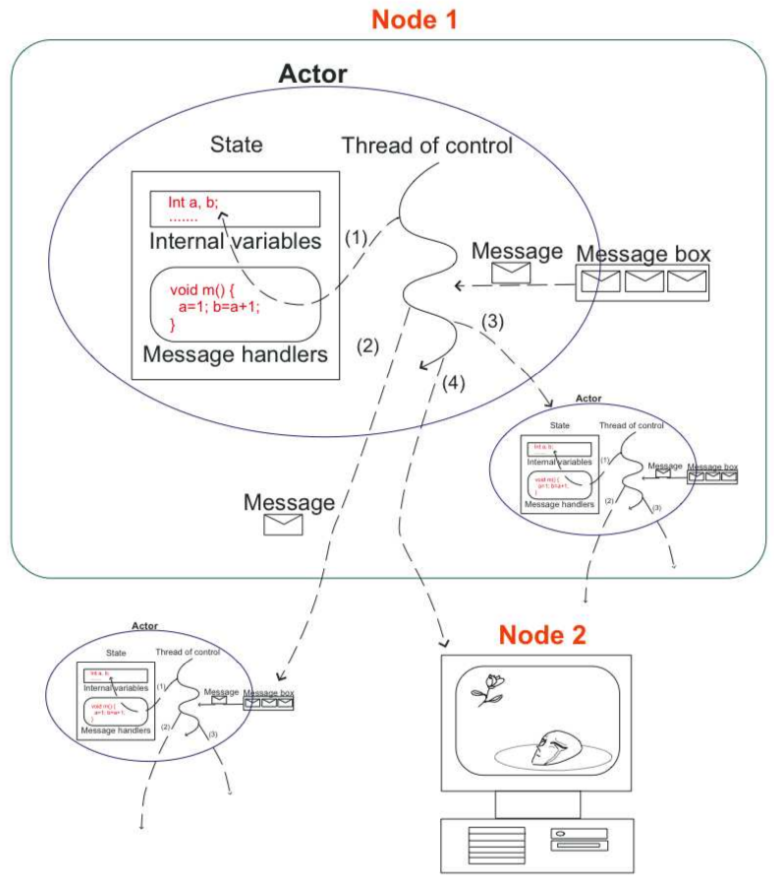
\includegraphics[width=0.5\textwidth]{Actors.png}
\caption{\label{fig:actors}Actors are reactive entitites. In response to a message, an actor can (1) change its internal state, (2) send messages to peer actors, (3) create new actors, and/or (4) migrate to another computing host}
\end{figure}

For our implementation of the chat application, we use SALSA (Simple Actor Language, System and Architecture)~\cite{Varela:2001:PDR:583960.583964} as our actor language. It is an actor-oriented programming language designed and implemented to introduce the benefits of the actor model while keeping the advantages of object-oriented programming. SALSA is a dialect of Java, and it is intended to reuse as many features of Java as possible. Abstractions include active objects, asynchronous message passing, universal naming, migration, and advanced coordination constructs for concurrency. SALSA is pre-processed into Java and preserves many of Java’s useful object oriented concepts- mainly, encapsulation, inheritance, and polymorphism. SALSA abstractions enable the development of dynamically reconfigurable applications. A SALSA program consists of universal actors that can be migrated around distributed nodes at runtime.\\ 

In order to support execution of SALSA applications on Android, we ported SALSA runtime to the Android platform.~\cite{salsaandroid} provides the instructions for setting up the runtime so we can run SALSA applications compiled to JVM bytecode. It involves setting up a universal naming service that allows setting up universal actors which can migrate across physical resources. Once the nameserver is up, we setup theaters on the smartphone and servers where migration should be enabled. Theaters are a set of virtual machines that host one to many concurrently running universal actors. Theaters provide a layer beneath actors for message passing, remote communication, and migration. Every theater consists of a RMSP (Remote Message Sending Protocol) server, a local cache that maps between actors’ names and their  current locations, a registry that maps local actor names to their references, and a run-time environment. The RMSP server listens for incoming requests from remote actors and starts multiple threads to handle incoming requests simultaneously.

% The most successfully scalable chat room applications (those involving tens of millions of users) have been
% written in an actor language. 

\section{Common language for interoperability with SALSA}
We had to identify a language that would provides the required abstractions for designing friendly user interfaces for our chat application, and at the same time provide interoperability with SALSA actors. Ideally, the two languages should compile down to run on a single execution engine so that the interface layer for communication between the two languages is efficient. This led us to using Kotlin~\cite{kotlin} as our common intermediate language. It is interoperable with Java and Android, making it an ideal candidate for our requirements.\\

Kotlin is a statically typed programming language for multiplatform applications. It is a great fit for developing server-side applications, allowing to write concise and expressive code while maintaining full compatibility with existing Java-based technology stack and a smooth learning curve: 
\begin{itemize}
\item \textbf{Expressiveness}: Kotlin's language features, such as its support for type-safe builders and delegated properties, help build powerful and easy-to-use abstractions
\item \textbf{Scalability}: Kotlin's support for coroutines helps build server-side applications that scale to massive numbers of clients with modest hardware requirements.
\item \textbf{Interoperability}: Kotlin is fully compatible with all Java-based frameworks, which lets you stay on your familiar technology stack while reaping the benefits of a more modern language.
\end{itemize}

It is also a great fit for developing Android applications, bringing all of the advantages of a modern language to the Android platform without introducing any new restrictions:
\begin{itemize}
\item \textbf{Performance}: A Kotlin application runs as fast as an equivalent Java one, thanks to very similar bytecode structure. With
Kotlin's support for inline functions, code using lambdas often runs even faster than the same code written in Java.
\item \textbf{Interoperability}: Kotlin is 100\% interoperable with Java, allowing to use all existing Android libraries in a Kotlin application. This includes annotation processing, so databinding and Dagger work too.
\end{itemize}

\section{Toolchain}
We leverage the fact that SALSA and Kotlin both compile down to JVM bytecode, in order to build a toolchain for compiling Kotlin/SALSA applications. This allows us to use a single execution engine without incurring the cost of IPC for communication between the SALSA and Kotlin language environments. Figure~\Figref{toolchain} shows the steps for building the source files in Kotlin and SALSA to execute on Android. Note that the Java interface file is also compiled with the other Java sources to JVM bytecode for communicating between SALSA and Kotlin environments. 

\begin{figure}
\centering
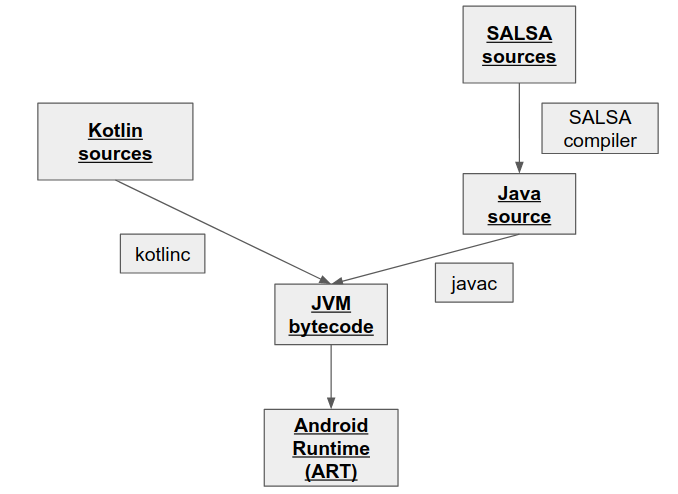
\includegraphics[width=0.8\textwidth]{toolchain.png}
\caption{\label{toolchain}Toolchain and flow for compiling Kotlin and SALSA code to execute on Android runtime (ART)}
\end{figure}

\section{Interface design}
We design an interface for translating the Kotlin bytecode to Java. To show how this works, let's say the user of chat application registers with the server, and so a client machine is created as per the network model in Figure~\Figref{fig:spec}. A record for the user is also stored, using the data model. Once presented with a simple graphical user interface on her smartphone (such as the one shown in ~\Figref{fig:chat}), the user now has the ability to trigger events. 
\begin{figure}
\centering
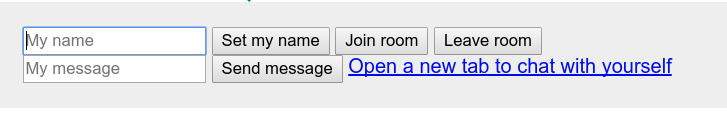
\includegraphics[width=0.8\textwidth]{Chat.png}
\caption{\label{fig:chat}Basic chat window with supported events}
\end{figure}

For each button, a corresponding event is triggered in the event model (Join room button triggers a JoinRoom event) which generates a message passed to a singleton object in Java. The message contains the actor name for the SALSA actor responsible for processing JoinRoom event, along with arguments such as client and server instances, and the ChatRoom instance that the user intends to join. Using Java reflection APIs, we translate this request from Kotlin, to a message being sent to JoinRoom actor in  SALSA domain. The arguments provided are included in the message sent to JoinRoom actor. The actor then proceeds with implementing the logic contained in the event model definition, such as updating the room's members with the new user sending the request. 

Using a generic interface in Java allows for having a single separation layer that manages communication between Kotlin and SALSA environments. It processes all Kotlin requests and redirecting them to corresponding SALSA actors with required arguments in message content.~\Figref{fig:clientserver} shows a high level overview of the system with the Java interface sitting between Kotlin and SALSA layers on each client machine. 

\begin{figure}
\centering
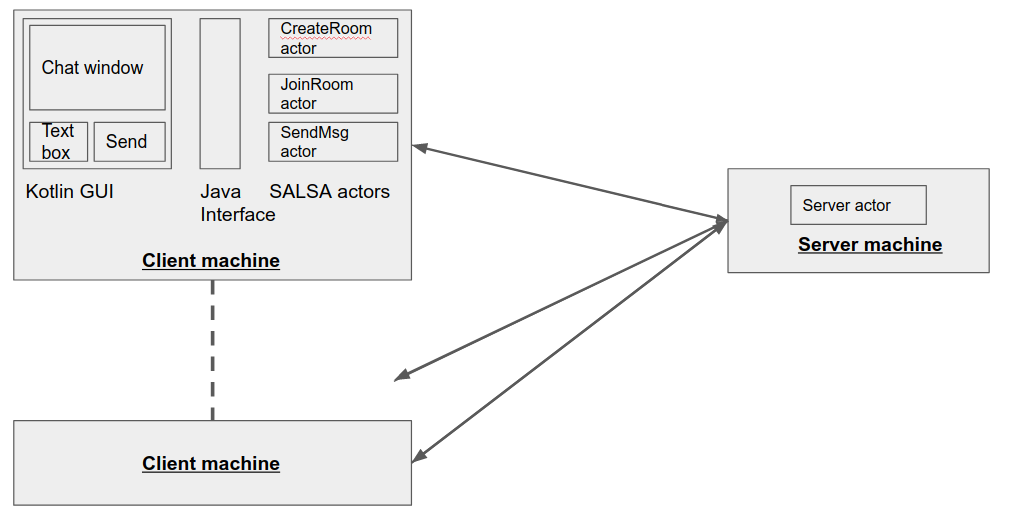
\includegraphics[width=0.8\textwidth]{Client-Server.png}
\caption{\label{fig:clientserver}High level overview of chat application across client/server machines. The Kotlin GUI interacts with SALSA actors via common Java interface. The Kotlin client sends requests with arguments such as user registration, chat message send, chat message receive. These requests are translated to actor messages via SALSA layer and sent to server actor. The server actor in turn sends messages to the client actor, such as chat message update (for message broadcast functionality), registration status and chat message receive.}
\end{figure}


\section{Results}

We have successfully built a chat application which has its GUI written in Kotlin, whereas all the chat message handling (including registration, send and broadcast to all clients) is done in the SALSA layer. We have been able to execute the entire system on a single execution engine within each client. This helps us avoid any additional IPC overhead for message passing and manage switching between multiple environments. The following related code has been hosted online: 
\begin{itemize}
\item ~\cite{salsaandroid} shows the steps for running SALSA code on Android 
\item ~\cite{chatapp} has sample code and build steps for executing 2 chat clients interacting with a server. 
\end{itemize}

We are currently working on fully automating the translation of the user level language, as shown in Figure~\Figref{fig:spec}, into Kotlin and corresponding SALSA code that represents the data model, network model and event models.

\section{Future work}
Once we have an automatic translation layer and generic interface for communication between Kotlin and SALSA layers in our chat application, we intend to demonstrate the capability of the infrastructure we have built, in a different application domain. We are considering object spreadsheets~\cite{McCutchen:2016:OSN:2986012.2986018} or collaborative text editing for this purpose.  

% \subsection{How to include Figures}

% First you have to upload the image file from your computer using the upload link the project menu. Then use the includegraphics command to include it in your document. Use the figure environment and the caption command to add a number and a caption to your figure. See the code for Figure \ref{fig:frog} in this section for an example.


% \subsection{How to add Comments}

% Comments can be added to your project by clicking on the comment icon in the toolbar above. % * <john.hammersley@gmail.com> 2016-07-03T09:54:16.211Z:
% %
% % Here's an example comment!
% %
% To reply to a comment, simply click the reply button in the lower right corner of the comment, and you can close them when you're done.

% Comments can also be added to the margins of the compiled PDF using the todo command\todo{Here's a comment in the margin!}, as shown in the example on the right. You can also add inline comments:

% \todo[inline, color=green!40]{This is an inline comment.}

% \subsection{How to add Tables}

% Use the table and tabular commands for basic tables --- see Table~\ref{tab:widgets}, for example. 

% \begin{table}
% \centering
% \begin{tabular}{l|r}
% Item & Quantity \\\hline
% Widgets & 42 \\
% Gadgets & 13
% \end{tabular}
% \caption{\label{tab:widgets}An example table.}
% \end{table}

% \subsection{How to write Mathematics}

% \LaTeX{} is great at typesetting mathematics. Let $X_1, X_2, \ldots, X_n$ be a sequence of independent and identically distributed random variables with $\text{E}[X_i] = \mu$ and $\text{Var}[X_i] = \sigma^2 < \infty$, and let
% \[S_n = \frac{X_1 + X_2 + \cdots + X_n}{n}
%       = \frac{1}{n}\sum_{i}^{n} X_i\]
% denote their mean. Then as $n$ approaches infinity, the random variables $\sqrt{n}(S_n - \mu)$ converge in distribution to a normal $\mathcal{N}(0, \sigma^2)$.


% \subsection{How to create Sections and Subsections}

% Use section and subsections to organize your document. Simply use the section and subsection buttons in the toolbar to create them, and we'll handle all the formatting and numbering automatically.

% \subsection{How to add Lists}

% You can make lists with automatic numbering \dots

% \begin{enumerate}
% \item Like this,
% \item and like this.
% \end{enumerate}
% \dots or bullet points \dots
% \begin{itemize}
% \item Like this,
% \item and like this.
% \end{itemize}

% \subsection{How to add Citations and a References List}

% You can upload a \verb|.bib| file containing your BibTeX entries, created with JabRef; or import your \href{https://www.overleaf.com/blog/184}{Mendeley}, CiteULike or Zotero library as a \verb|.bib| file. You can then cite entries from it, like this: \cite{greenwade93}. Just remember to specify a bibliography style, as well as the filename of the \verb|.bib|.

% You can find a \href{https://www.overleaf.com/help/97-how-to-include-a-bibliography-using-bibtex}{video tutorial here} to learn more about BibTeX.

% We hope you find Overleaf useful, and please let us know if you have any feedback using the help menu above --- or use the contact form at \url{https://www.overleaf.com/contact}!

\bibliographystyle{alpha}
\bibliography{sample}

\end{document}